\documentclass[a4paper, 11pt]{article}
\setlength{\topmargin}{0.0in}
\setlength{\textheight}{9.5in}
\setlength{\oddsidemargin}{-.1in}
\setlength{\textwidth}{6.5in}
\usepackage{parskip}
\usepackage{graphicx}
\graphicspath{ {images/} }

\usepackage{datetime}
\usepackage[font={small,it}]{caption}
\usepackage{listings}

\newdateformat{monthyeardate}{%
  \monthname[\THEMONTH], \THEYEAR}

\date{}
\begin{document} 

\LARGE\title{Real Time Tempo Analysis of Drum Beats}

\LARGE\author{Author: \textbf{Philip Hannant}, Supervisor: \textbf{Professor Steve Maybank}\\
\\Birkbeck, University of London\\
Department of Computer Science and Information Systems\\
\\Project Report\\
MSc Computer Science\\
\\\monthyeardate\today
}





\normalsize


\maketitle
\newpage
\tableofcontents
\clearpage

\section*{Abbreviations}
\begin{tabular}{l p{4.5in}  }\\
\textbf{BPM} & Beats Per Minute\\
\textbf{DWT} & Discrete Wavelet Transform\\
\textbf{FFT} & Fast Fourier Transform\\
\textbf{JSON} & Javacript Object Notification\\
\textbf{IDE} & Integrated Development Environment\\
\textbf{TDD} & Test Driven Development\\
\end{tabular}

\section*{Definitions}
\begin{tabular}{l p{4.5in}}\\
\textbf{Acoustic Drum Kit} & A collection of drums and cymbals which do not have electronic amplification. Typically made up of a bass drum, snare drum, tom-toms, hi-hat and 1 or more cymbals.\\\\
\textbf{Beat} & For the purpose of this project a beat will be defined as the sequence of equally spaced pulses used to calculate the tempo being played by the drummer.\\\\
\textbf{Downbeat} & Refers to beat one of a measure of music, called a downbeat to correspond to the motion a conductor's arm [1].\\\\
\textbf{Drum Module} & The device which serves as a central processing unit for an electronic drum kit, responsible for producing the sounds of the drum kit.\\\\
\textbf{Electronic Drum Kit} & An electrical device which is played like an acoustic drum kit, producing sounds from a stored library of instruments and samples.\\\\
\textbf{MIDI} & Musical Instrument Digital Interface is a protocol developed in the 1980's to allow electronic instruments and other digital musical tools to communicate with each other [3].\\\\
\textbf{Tempo} & The speed at which a piece of music is played \cite{oxford-comp} and counted in beats per minute (bpm).\\\\
\end{tabular}
\clearpage

\maketitle{} \section{Introduction and Background}

This project report presents my aim to develop a real-time drum beat tempo analysis system using different beat detection algorithms which is able to record the perfomance of each method concurrently when an extensive set of drum samples, representing a real drummer's perfomance, is processed through the system.

\subsection{Drumming Training Tools Background}
Timing is the fundamental skill any good drummer should possess and is the staple by which they will be judged. For many years the only training tool available to a drummer to improve their timing was the metronome. An instrument used to mark musical tempo, erroenously attributed to Johann Nepomuk Maelzel in 1815 but was actually invented by a Dutchman, Dietrich Nikolaus Winkel a year earlier. The traditional metronome, based on Winkel's original design is a hand-wound clockwork instrument that uses a pendulum swung on a pivot to generate the ticking which depicts the desired tempo \cite{brit-metro} is still used today by musicians, as seen in Figure~\ref{fig: TradMet}. \par

\begin{figure}[ht]
	\centering
	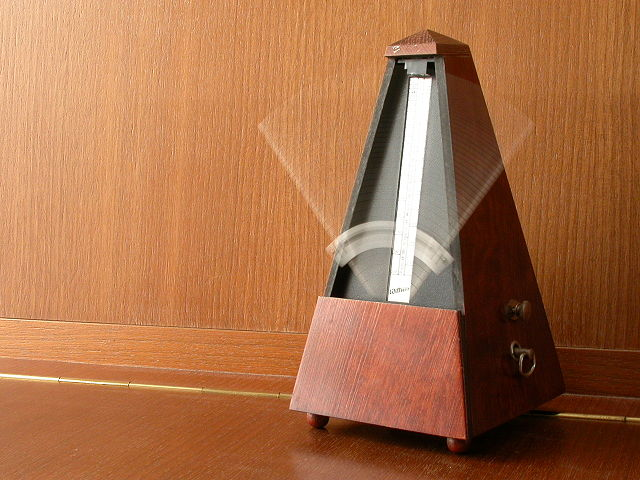
\includegraphics[scale=0.30]{TradMet}
	\caption{Traditional Metronome}% (Source: https://commons.wikimedia.org/w/index.php?curid=1058005)}
	\label{fig: TradMet}
\end{figure}

For drummers however the electronic versions of the metronome are much more widely used, to the point that metronomes are now developed with functionality specifically tailored to a drummers training requirements. The Tama Rhytham Watch (Figure~\ref{fig: RW200}) was the first metronome designed specifically for drummers, providing enough volume to be used with real drums as well as allowing for the use of different time signatures and preset set rhythm patterns to help improve perfomance.\par
\clearpage

\begin{figure}[ht]
	\centering
	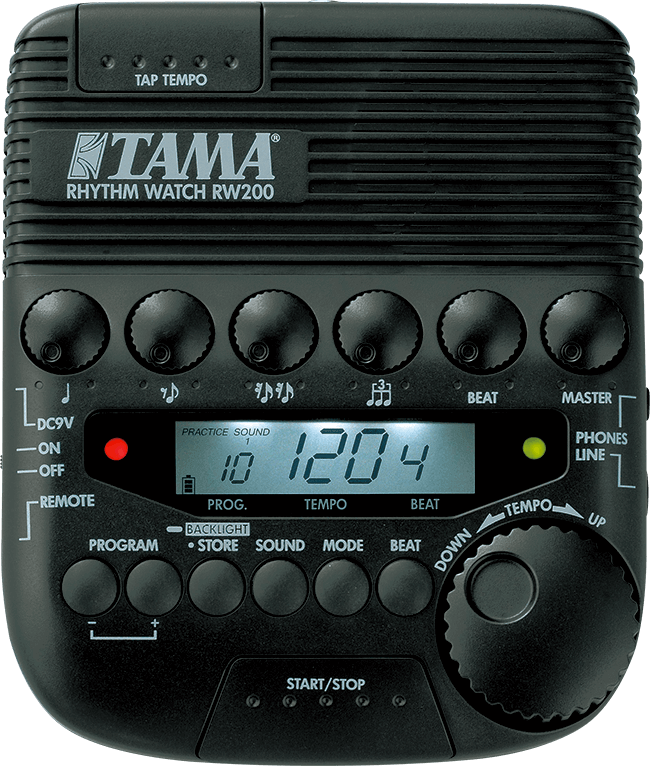
\includegraphics[scale=0.25]{RW200}
	\caption{Tama Rhythm Watch}% (Source: http://www.tama.com/eu/products/accessories/RW200.html)}
	\label{fig: RW200}
\end{figure}

Following the development of MIDI driven electronic drum kit came the development of more advanced training tools that now were able to provide live feedback to drummer during any given perfomance. Today the leaders in this field are Roland, their v-drums line provide a variety of tutition packages including the SCOPE and more recently the COACH system provided in the v-drum modules, the v-drum Rhymthm Coach line is an advanced version of the traditional drummers practice pad and the extensive DT-1 V-Drums tutor software package. Roland have even now gamified this field with their latest release, the V-Drums Friend Jam app. The application itself provides the player with live feedback and evaluates each performance in order to provide the player with a score which they can share over social media. \par

The aim of this project is to investigate whether some of the current beat detection algorithms available would be accurate enough to provide the basis for a training tool for dummers using an acoustic drum kit as opposed to an electronic drum kit. \par

\subsection{Drum Musical Theory}
In order to understand the fundamentals of musical timing some theory needs to be examined but beforehand the concept of a drummer playing time must be considered. Time, in a drumming sense is an informal term used to describe the consistent rhythmic pattern that a drummer will play on the hi-hat or ride cymbal \cite{drum-bible} and it can be considered one of the most important components of any drum beat. 

\subsubsection{Notation}
Drum music notation is written on staff that is made up of five individual lines, the clef is found on the far left of the staff which indicates the pitch of the notes \cite{oxford-comp} and as percussion instruments are non-pitched they use the percussion-clef. On traditional musical notation the lines and spaces between represent a tonal where as for drum notation, notes written on lines or spaces indicate a certain drum or cymbal. The staff is seperated into individual measures which are known as bars \cite{drum-note} and it is these bars that are the basis of musical time. For the purpose of this project it is the count of these beats that will be used to calculate the tempo of a certain drum beat.

\subsubsection{Time Signatures}
Time signatures appear on the staff just after the clef and are written as a fraction where the top number indicates the number of beats that there are in a bar. With the bottom number representing the size of the note that makes up the duration of one beat. For example the straight time four four (4/4) or common time signature indicates four beats in each bar or measure where each beat is made up of one quarter note \cite{drum-note}. Within these bar lines beats can be further divided by using a technique known as subdivision, which is a method for reducing the pulse or rhythm pattern into smaller parts than those originally written, for example counting a four four (4/4) measure in eighth (1/8) or sixteeth (1/16) notes. 

\subsubsection{Notes}
The notes used to represent the percussive instrument to be played also provide the duration it should be played for. Notes come in different lengths and the key values are the whole (1/1), half (1/2), quarter (1/4), eighth (1/8) and sixteeth (1/16). For example two eighth notes represent the same time value as a single quarter note. It is possible to divide a note values by three instead of two, these notes are known as triplets. An eighth note triplet is played fifty percent faster than a normal eighth note, therefore for every two eighth notes there will be three eighth note triplets \cite{drum-note}. An example of the eighth-note triplets being used is in a twelve eight (12/8) jazz shuffle, the time element played on the ride cymbal or hi-hat is charaterised by playing the first and third triplet of an eighth-note triplet grouping \cite{drum-bible}.

\subsubsection{Playing Basics}
With the basics of drum theory covered it is now possible to discuss the key elements of a drum beat, typically for a straight four four (4/4) bar the bass drum will be played on the first and third beat and the snare drum will be played on the second and forth beat both as quarter notes. This is more commonly known as a back beat \cite{drum-bible}. This just leaves the time element which will usually be played on the ride cymbal or hi-hat, this too could be played using quarter notes on the first, second, third and forth beats. However, in order to make the drum pattern more dynamic the time element will usually be played using subdivisions, typically using eighth note subdivisions. The ride cymbal or hi-hat will therefore be played on the first, second, third and forth beats as well as the eighth notes inbetween each quarter note. This can be demostrasted by counting the one-and-two-and-three-and-four-and, where the and represents the subdivided eighth note. Additonally to this technique a drummer will usually ensure that there is difference in the volume of the eighth notes being played on the quarter notes and those being played on the and. This technique of emphasising certain beats is known as accenting. 


\subsection{Beat Detection Background}
Most of the early work on beat detection was a by-product of research directed at other areas of musicical understanding. The earliest work in this field can be attributed to H. C. Longuet-Higgins, who in 1976 while researching the psychological theory of how Western musicians perceive rhythmic and tonal relationships between notes. Produced an algorithm that was able to follow the beat of a performance and adjust the perceived tempo accordingly based on whether a note started earlier or later than expected \cite{allen-danneburg}. Longuet-Higgins' work was built on the premise that in order to percieve the rhythmic structure of a melody it is first necessary to identify the time at which each beat occurs \cite{longeut1}, otherwise know as onset detection. The onset of a note is the instant which marks start of the variation in the frequency of a signal, a visualisation of this can be seen in Figure~\ref{fig: Onset}. Once detected it can then be used to measure the onset times of sonic events\footnote{A sonic event is a singular feature of a piece music which can be made up of one source or many\cite{sonic}, e.g. the hitting of a drum} within a piece of music\cite{mirex-onset}. These onset times are then used within a beat detection algorithm in order to calculate the piece of music's tempo. 

\begin{figure}[ht]
	\centering
	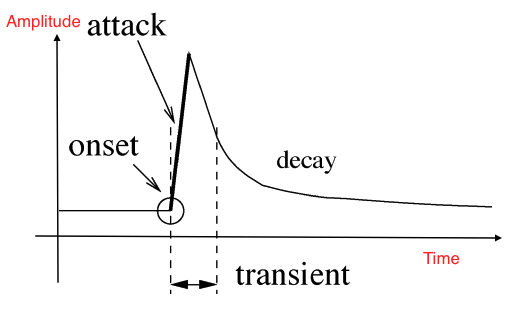
\includegraphics[scale=0.40]{Onset}
	\caption{The onset of a note is the instant which marks start of the variation in the frequency of a signal (Image Source: \cite{onset-tut})}
	\label{fig: Onset}
\end{figure}

Since Longuet-Higgins' first work the are of beat detection has expanded rapidly, in 2005 the first annual Music Information Retrieval Evaluation eXchange (MIREX) was held in 2005. MIREX includes a contest with the goal of comparing state-of-the-art algorithms for music information retrieval \cite{mirex-main}. The topics to be evaluated are proposed by the participants. In the first year, three of the nine topics concerned beat detection, including audio onset detection and since it's first inclusion it has been an evalulated topic of all but one of the last twelve contests \cite{mirex-onset}. The beat detection algorithms proposed to perform the tempo analysis for this project, the Beatroot system developed by Simon Dixon \cite{dixon1} and a development on the original audio analysis using the Discrete Wavelet Transform (DWT) by Tzanetakis, Essel and Cook \cite{tzane1}. Are both former entrants the MIREX contest, with the beatroot system receiving the highest score in the 2006 Audio Beat Tracking task \cite{mirex-06} 

\subsection{Project Aims}
The primary aim of this project is to investigation whether some of the currently avaliable beat detection algorthims are accurate enough to form the basis for a training tool to be used by drummers practicing on an acoustic drum kit. In order to achieve this the developed software package, hereafter referred to as  RTT\_Analyser\footnote{Where RTT stands for Real Time Tempo}, will need to process enough live audio in form of preconstructed drum beats and record each of the chosen beat detection algorithms accuracy. 

The original core features of the RTT\_Analyser developed for this project are:

\begin{enumerate}
\item A live audio tempo analysis tool, that compares and records the performance of selected beat detection algorithms
\item The RTT\_Analyser implements an adapted version of the beat tracking system Beatroot and Discrete Wavelet Transform algorithm described by Tzanetakis \textit{et al}'s\cite{tzane1} which process live audio as opposed to originally designed off-line audio files.
\item RTT\_Analyser implements a concurrent system that provides the same captured live audio data to the chosen beat detection algorithms in order for the tempo to be calculated simultaneously.
\item While processing live audio the RTT\_Analyser stores a predetermined data set in order to allow for performance analysis of the beat detection algorithms.
\item The RTT\_Analyser will provide the user with real time feedback of the most recent tempo calculation returned
\item In order to An extensive sample set of drum beats will need to be created to ensure the system is tested sufficiently
\end{enumerate}



\maketitle{}\section{RTT\_Analyser Beat Detection Algorthims}
The original proposed solution incorporated two beat detection algorithms, Beatroot system \cite{dixon1} and the DWT method \cite{tzane1}. However during the development the adaptation of the Beatroot system to be used with live audio took longer than the proposed time-frame. This meant that an alternative system needed to be found in order to mitigate this issue, conveniently the Beatroot software package also contained another beat detection system, the Performance Worm \cite{dixon3}. In order to ensure the project remained on track it was decided to substitute the Performance Worm for the Beatroot system. The intention was, if time allowed, to resume the adaptation of the Beatroot system to work with live audio once the project was ahead of schedule and this was successfully completed prior to the development of the user interface.

The project report will now discuss all of the beat detection algorithms that were incorporated in the RTT\_Analyser as well as the system used to allow for simultaneous tempo calculation.  

\subsection{Beatroot}
Beatroot is a beat detection software package created by Simon Dixon \cite{dixon1}, which was originally designed extract musical expression information musical recordings\cite{dixon3}. Beatroot was included in the RTT{\_}Analyser as the algorithm designed by Dixon was considered to be sufficiently fast enough to be implemented as part of a real-time system\cite{dixon4}.\par

Beatroot works by first obtaining a time-frequency representation of the signal based on a Short Time Fourier Transform (STFT) using a Hamming window\cite{dixon2}. The STFT is a form of Fourier transform (FT), which can be used to find out how much of each frequency exists in a signal. Th A negative of the FT is that it is unable to provide any details of when a frequency component occurs in time for non-stationary signals\footnote{Non-stationary signals are signals whose frequency contents changes over time\cite{polikapt2}}. A solution to this is to split a non-stationary signal up into a number of smaller segments using a window function, which effectively created a series of stationary\footnote{The frequency contents of a stationary signal does not change over time} signals which the FT could then be applied to. By splitting the signal into smaller segments the STFT is able to apply the DFT to these segments and essentially express a signal as a linear combination of elementary signals that are easily manipulated. The DFT returns a spectrum that contains information about how the energy held within the signal is distributed in the time and frequency domains\cite{tzane2}. The use of a Hamming window function in the STFT employed by Beatroot is an attempt to reduce the amount of additional frequencies appearing in the returned DFT spectrum, known as spectral leakage, which is caused when the steep sloped of the a rectangular window causes the frequecies to become distorted. The Hamming window counteracts this by using a bell shape, which has the effect of reducing amplitudes of its sidelobes\cite{lyons} and ensures the spectrum returned is less spread out and closer to the ideal theoretical result\cite{tzane2}. A visualisation of a Hamming window can be seen in Figure~\ref{fig: hamWin}. 

\begin{figure}[ht]
	\centering
	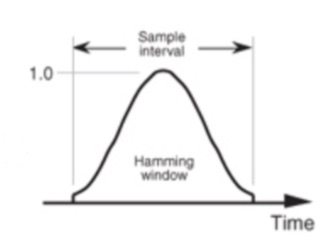
\includegraphics[scale=0.36]{hamWin}
	\caption{(Image Source: \cite{lyons})}
	\label{fig: hamWin}
\end{figure}

Once the time-frequency representation is returned the next stage is to the spectral flux onset detection function, which is a method for measuring the change in magnitude of each returned frequency bin\cite{dixon2}. The onsets are then selected from the spectral flux onset detection function by a peak-picking algorithm which finds local maxima within the detection function. The next stage is to apply the tempo induction algorithm which is used to compute clusters of inter-onset intervals (IOI) by using the calculated onset times. Each cluster represents a hypothetical tempo, in seconds per beat \cite{dixon1}. The clustering algorithm works by assigning an IOI to a cluster if its difference from the cluster is less than 25ms. The cluster information is then combined by recognising the approximate integer relationships between clusters. An example of this can be seen in Figure~\ref{fig: br-clusters} where cluster C2 is twice as long as C1 and C4 is twice that of C2. This information along with the number of IOIs within a cluster is then used to weight each cluster which is then returned as a ranked list of tempo hypotheses\cite{dixon4}.

\begin{figure}[ht]
	\centering
	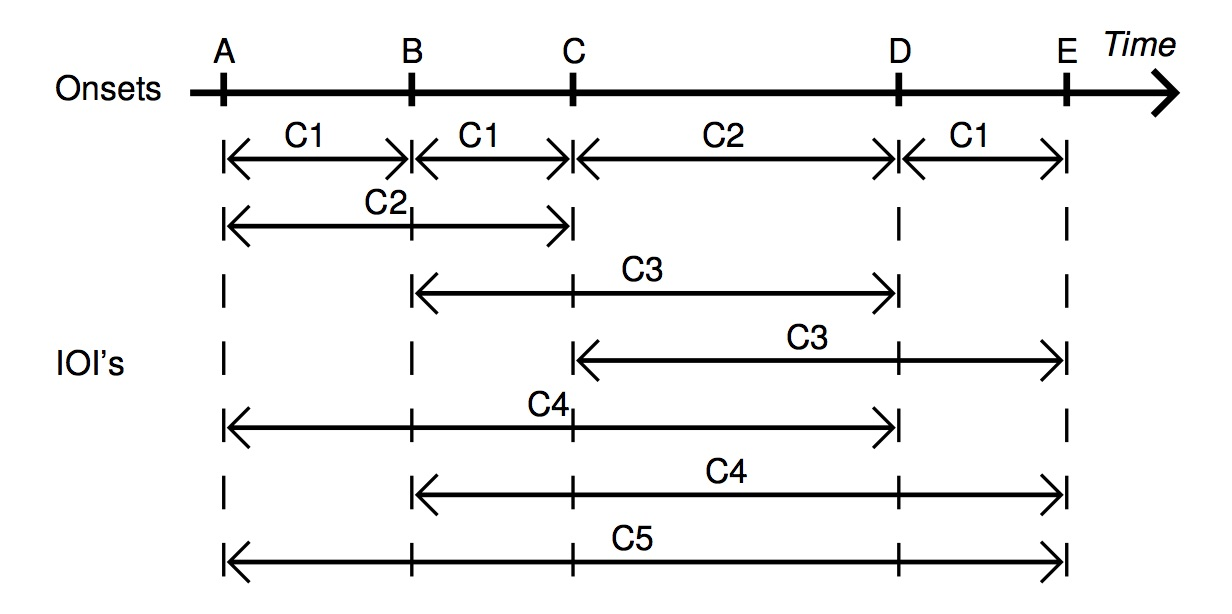
\includegraphics[scale=0.25]{br-clusters}
	\caption{(Image Source: \cite{dixon4})}
	\label{fig: br-clusters}
\end{figure}

The multiple agent architecture of Beatroot's beat tracking subsystem is then employed to find the sequences of events that closest match the original tempo hypotheses, each of these sequences is then rated and the most likely set of beat times is determined. Each of the agents in initialised with a tempo or beat rate hypothesis and an onset time. Further beats are then predicted by the agent based on these parameters. Any onsets corresponding with the predicted beat times are taken as a beat time, while those that fall outside of the are considered not to be a beat time, although the possibility that the onset is not on the beat is considered. Then agents then rate themselves based on an evaluatio function which looks at how evenly spaced the beat times are, the number of predicted beats which relate to actual events, and the salience\footnote{The salience is a measure of the note duration, density, pitch and density\cite{dixon1}, which is calculated from the spectral flux of the onset\cite{dixon4}} of the matched onsets. The agent with the highest score is then returned as the sequence of beats corresponding to the processed audio\cite{dixon4}. It is from the sequence of beats which this agent returns that overall tempo of the audio can be determined by using the ``inter-beat intervals, measured in beats per second''\cite{dixon1} to calculate beats per minute (bpm) of the audio.


\subsection{Discrete Wavelet Transform and Beat Detection Method}
The first literature regarding the wavelet was provided by the mathematician Albert Haar in 1909 [18]. The wavelet transform is a technique for analysing signals which was developed as an alternative to the STFT\cite{tzane1}. Like the STFT, the DWT is able to provide time and frequency information, however, unlike the STFT the DWT is able to do this without the need for a window function. The DWT can essentially be considered to be a filterbank, where a filterbank is a system used to separate subbands by using an array or bank of filters, where each of the filters corresponds to half frequency range of the closest centre higher frequency. Thus each filter will have half or twice the bandwith of any of its adjacent filters. 

In 2001, Tzanetakis \textit{et al} described how the Discrete Wavelet Transform (DWT) could be used to extract information from non-speech audio\cite{tzane1}. Their beat detection algorithm was based on the detecting the most prominent signals which are repeated over a period of time within the analysed audio. The first stage is to process is to split the signal into a number of octave\footnote{define an octave} frequency bands with the DWT. This allows for the time domain amplitude envelopes of each frequency band to be extracted separately. The extraction of these envelopes is completed in the following three steps:

\begin{enumerate}
\item Full Wave Rectification - process of converting the amplitude of each frequency band to one polarity\cite{pallas}, which can be either positive or negative. A visual representation can be seen in Figure~\ref{fig: fwr}.
\item Low Pass Filtering - Low pass filtering is a signal processing technique which is designed to allow frequencies below a cutoff frequency through but blocks any frequencies above the cutoff frequency\cite{smith}.
\item Downsampling - Due to the large perodicities that can occur in beat analysis, downsampling the signal reduces the computation time of the autocorrelation stage without causing any negative effects on the performance or the algorithm\cite{tzane3}
\end{enumerate}

\begin{figure}[ht]
	\centering
	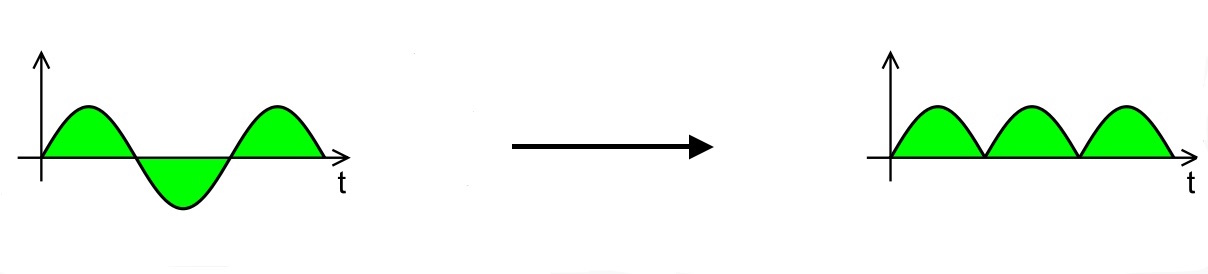
\includegraphics[scale=0.25]{FWR2}
	\caption{Visual representation of Full Wave Rectification (diagram adaptedfrom https://en.wikipedia.org/wiki/Rectifier)}
	\label{fig: fwr}
\end{figure}


After these steps each frequency band os normalised through a method of mean removal in order to ensure the signal is centred at zero for the autocorrelation stage. The autocorrelation function is then applied to each frequency band and its peaks correspond to the various periodicities of that signal's envelope. The first five peaks of the function and their corresponding periodicities are then calculated in beats per minute and added to a histogram, this process is repeated while iterating over the signal. The estimated tempo of the audio signal is then retrieved from the periodicity that corresponds to the highest peak within the histogram\cite{tzane1}.

Originally, it was intended that Discrete Wavelet Transform beat detection component of the RTT\_Analyser would be implemented by the author. It was recognised in the project proposal that this could result in the rest of the project being delayed and therefore a mitigation to adapt the Matlab implementation of the Tzanetakis \textit{et al}\cite{tzane1} algorithm by Eng Eder de Souza\cite{desouze}. Due to the time spent in investigating how to adapt the Beatroot system to work with live audio a different solution was needed, this was provided by the Scala implementation by Marco Ziccardi\cite{marcoZin}.

\subsection{Performance Worm}
The final beat detection algorithm employed in the RTT\_Analyser is the Performance Worm (PW) system, designed by Simon Dixon, Werner Goebl and Gerhard Widmer\cite{dixonGoeblWidmer}. The PW is based on a real time algorithm which is able to determine the tempo of the input raw audio, while keeping track of other possible tempo hypotheses that are rated and updated dynamically. Allowing for the most recently highest ranked tempo hypothesis to be returned to the user\cite{dixonGoeblWidmer}. 

First the PW processes the raw audio which can either taken from a static recording or directly from a live input with a smoothing filter in order to obtain the RMS amplitude of the signal taken from a 40ms window (explain RMS and smoothing filter). The note onsets are then calculated by the event detection module that finds the slope of the smoothed amplitude and then calculates the set of local peaks which are taken as the note onset times\cite{dixonGoeblWidmer}. 

The signal is then processed by the multiple tempo tracking subsytem which uses a similar approach to the beatroot system. The time intervals (inter-onset intervals or IOIs) of event pairs are first calculated. A clustering algorithm (Figure~\ref{fig: clusterAl}) is then applied in order to determine the significant clusters of IOIs, which are subsequently assumed to be the musical units held within the signal. As in the beatroot system, these clusters are then used as the bases of the tempo hypotheses produced by the tempo tracking subsystem. While running the clustering algorithm keeps 5 seconds of onset times within memory and begins processing by determining all IOIs between the onsets in memory. The tempo inducer then explouts a property of most Western music where time intervals are related by small approximate interger ratios. As the times held by the clusters can be considered to represent related notes, e.g. quarter and eighth notes. The tempo inducer then adjusts cluster times and weightings according to the information held by the sets of related clusters. Two clusters are considered to be related if the ratio of their time intervals is close to an interger. The highest weighted clusters are their respective tempo hypothesis is then returned as the tempo output\cite{dixonGoeblWidmer}.


\begin{figure}
	\hspace{10mm} For each new onset\\
	\hspace*{20mm} For IOI times $\mathit{t}$ from 100ms to 2500ms in 10ms steps\\
	\hspace*{30mm} Find pairs of onsets which are $\mathit{t}$ apart\\
	\hspace*{30mm} Sum the mean amplitude of these onset pairs\\
	\hspace*{20mm} Loop until all IOI time points are used\\
	\hspace*{30mm} For times $\mathit{t}$ from 100ms to 2500ms in 10ms steps\\
	\hspace*{40mm} Calculate window size $\mathit{s}$ as function of $\mathit{t}$\\
	\hspace*{40mm} Find average amplitude of IOIs in window $\mathit{[t, t + s]}$\\
	\hspace*{40mm} Store $\mathit{t}$ which gives maximum average amplitude\\
	\hspace*{30mm} Create a cluster containing the stored maximum window\\
	\hspace*{30mm} Mark the IOIs in the cluster as used\\
	\hspace*{20mm} For each cluster\\
	\hspace*{30mm} Find related clusters (multiples or divisors)\\
	\hspace*{30mm} Combine related clusters using weighted average\\
	\hspace*{20mm} Match combined clusters to tempo hypotheses and update\\
	\caption{Clustering algorithm used in the Performance Worm Multiple Tempo Tracking Subsystem\cite{dixonGoeblWidmer}}
	\label{fig: clusterAl}
\end{figure}

\maketitle{} \section{Solution Design and Architecture}
The basic premise for the RTT\_Analyser is to enable the user to play a live drum beat through the system and the tempo of the live audio is returned to user as well as being stored for future analysis. Initially, the RTT\_Analyser opens the inbuilt microphone of the device upon which the software is being run. After establishing the live audio stream the RTT\_Analyser beat detection algorithms are sent the live audio data in the format of a byte array. These live audio bytes are then decoded according to the individual algorithm's requirements before being processed and the tempo calculated. A general schematic of the work-flow of the RTT\_Analyser can be seen in Figure (add in).

\subsection{Live Audio Processing}
The live audio is processed using the Javax Sound package. In order to make the results reflective of the quality of microphone that any future applications might use it was decided that the RTT\_Analyser was designed to be used with the built in to the device it was being executed on. In order to ensure the caputured audio matches CD quality the Javax Sound AudioFormat class was designed with the following constructors: 

\begin{itemize}
\item Encoding - This will be set to ``PCM.signed'', representing audio encoded to the native linear pulse code modulation, where pulse code modulation is the process of sampling and quantising the signal into discrete symbols for transmissions\cite{pulseWag}.
\item Sample Rate - 44,100, set to match CD quality for the number of analog samples which will be analysed per second. 
\item Sample Size in Bits - 24, based on a sound card with a 24 bit sample depth.
\item Channels - 2, audio will be captured using the built in microphone, typically stereo of the device the RTT\_Analyser is being run on.
\item Frame Size - 6, where the frame size is the number of bytes in a sample multiplied by the number of channels [17].
\item Frame Rate - 44,100, same as sample rate.
\item Big Endian (boolean) - false, as the project will be developed on an Intel core which uses a little-endian architecture\footnote{Endianess refers to the order of bytes which make up a digital word. Big endianess stores the most significant byte at a certain memory address and the remaining bytes being stored in the following higher memory addresses. The little-endian formate reverses the order storing the least significant at the lowest and most significant at the highest memory address [16].}.
\end{itemize}

The described audio format is then applied to the TargetDataLine, which provides access to the built in microphone of the device, if available. The TargetDataLine class is then attached to an instance of the Java AudioInputStream class which converts the captured audio into a stream of bytes for processing\cite{soundTrail}. In order to process the captured bytes the RTT\_Analyser then required the use of a concurrent system to allow for each of the three beat detection algorithms to be run in parallel, which was provided by the Akka Actors system.

\subsection{Akka Actors}
The Akka Actor Model is specifically designed to provide the ability to write concurrent systems with a high level of abstraction that alleviates the developer from the need to handle locking and individual thread management. Therefore, making it much easier to write concurrent and parallel systems when compared to the traditional approaches used in Java\cite{akkaActors}.

A fundamental construct of the Akka Actor system is that it strictly adheres too the Reactive Manifesto, which aims to ensure applications built under this are easier to develop and are amenable to change, allowing for a higher level of tolerance to failure and the ability to meet any such failure elegantly as opposed to disaster\cite{reactMan}. The Reactive Manifesto requires applications to satisfy one or more of the following requirements\cite{reactMan}:


\textbf{Responsive} - The system responds in a timely manner, if possible. By providing usability and utility responsiveness allows for any problems to be detected and resolved effectively.\\\\
\textbf{Resilient} - The system should be able to remain responsive even in the event of a failure, which applies to all parts of the system not just the mission critical components. To achieve this each component needs to be isolated within the system, therefore allowing failed parts of the system to recover without effecting the responsiveness of the system as a whole.\\\\
\textbf{Elastic} - The system will be able to maintain the same level of responsiveness despite varying workloads, reacting to changes in the rate of input by adapting the levels of resources allocated to service these inputs accordingly.\\\\
\textbf{Message Driven} - Reactive systems rely on the use of asynchronous message passing in order to establish boudaries between components within the system, ensuring isolation, loose-coupling\footnote{add one} and location transparency\footnote{add another}. By utilising a non-blocking\footnote{another!} message-passing it is possible to ensure message recipents only comsume resources when active, leading to a much reduced system overhead.\\\\


\subsubsection{The Actors}
The actors within the actor model are objects which are used to encapsulate state and behaviour. They communicate exclusively through messages passed to a recipients mailbox and it can help to in fact think of them as group of people being assigned subtasks within an organisational structure. One of the key features of an actor system is that tasks are split up and delegated until they become small enough to be handled in one piece. This process not only ensures that the tasks being carried out by the actors are clearly defined but also the actors themselves can be designed in terms of the mesaages they are able to receive and how they should react to these messages and any failures that might occur. The actors within a system will naturally form a set hierachy. For example, an actor system where an actor assigned the task of overseaing a certain function might split this function into a number of smaller tasks which it assigns some child actors that it supervises until the task is complete \cite{acotrsys}. The actors created within the RTT\_Analyser were a mix of stand alone actors and actors which were required to supervise subtasks carried out by child actors.

\subsection{Design Methods}
The design patterns used b     

\maketitle{} \section{Implementation}
The RTT\_Analyser is written in Java and Scala, due to the Beatroot and Peformance Worm both being written in Java, and the the author's familiarity with both languages and 

the Scala specific build tool, sbt (simple build too), which is a build tool that creates a stable build platform that increases productivity by utilising some good ideas from other build tools like, minimal configuration and built-in tasks including test, compile and publish. It is also able to support a reactive development environment that is able to re-run all tests when source code is updated\cite{sbt}. In terms of this project sbt was chosen as it supports mixed Scala/Java projects. Allowing for the Beatroot and Performance Worm systems written in Java to be easily incorporated with the Scala implementation of the Discrete Wavelet Transform and the Akka Actor system.

\subsection{Live Audio Capture}
To implement the RTT\_Analyser's live audio capture system the Javax Sound package was used. Initially, the SoundCaptureImpl class was created in Java to be responsible for the live audio capture and holding of the raw audio in a circular buffer before being processed by the respective beat detection algorithms. The sound capturing components of this class were based on those described in the Java Sound Programmer Guide\cite{javasound} and consisted of the code below:

\begin{lstlisting}
    private AudioFormat format;
    private TargetDataLine input;
    private DataLine dataLine;
    ...
        input = AudioSystem.getTargetDataLine(format);
        DataLine.Info info = new DataLine.Info(TargetDataLine.class, format);
        input = (TargetDataLine) AudioSystem.getLine(info);
        input.open(format); 
\end{lstlisting}

The need for the above code however became defunct with the design decision to include the Performance Worm system within the RTT\_Analyser as the Performance Worm was already set up to capture live audio. Therefore the captured audio now needed to be stored by the Performance Worm in a manner which allowed for all three beat detection algorithms to be able to process the same captured audio. This was achieved by adding the method \textit{addBytes} (Figure~\ref{fig: addBytes}) to the AudioWorm class, responsible for the capturing and processing of the live audio within the Performance Worm. The call to the \textit{addBytes} was added just below the \textit{.read} call of the AudioInputStream, the byte array was then passed to the \textit{addBytes} method and stored within a ByteArrayOutputStream to be processed later. The difference in processing windows of the Performance Worm to initally th

\begin{figure}[ht]
	\centering
	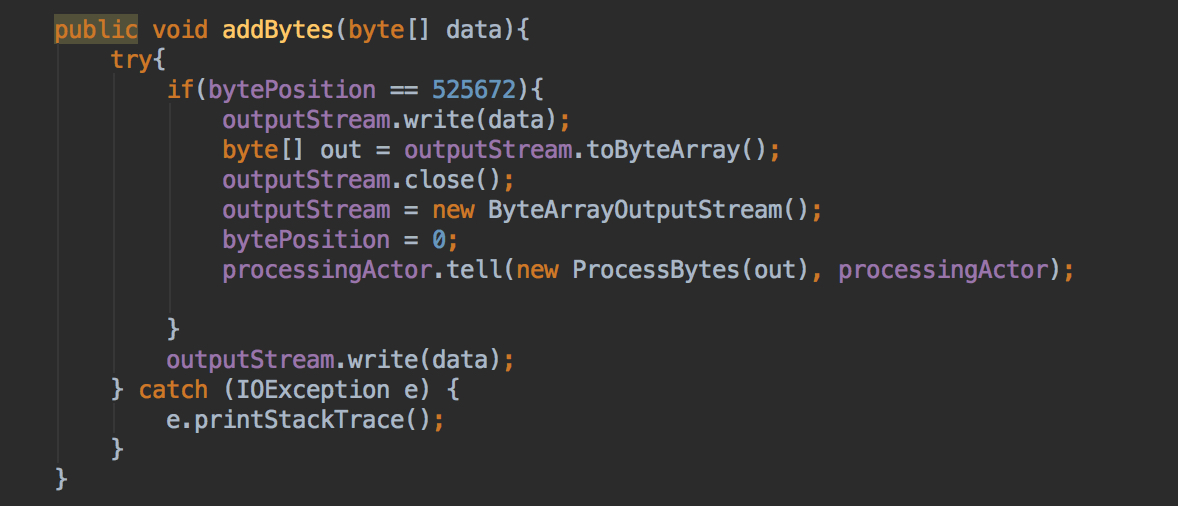
\includegraphics[scale=0.25]{images/addBytes.jpg}
	\caption{}
	\label{fig: addBytes}
\end{figure}

\subsection{DWT Beat Dectection Implementation}
The implementation of Tzanetakis \textit{et al} beat detection algorithm by Marco Ziccardi\cite{marcoZin} was part of a larger system which offered a number of other beat detection methods. The RTT\_Analyser only required the class which implemented the DWT beat detection algorithm, WaveletBPMDetector.\\

NEED SOME GLUE\\

The WaveletBPMDetector originally relied on a Scala version of the WavFile Java class created by Andrew Greensted\cite{green}, however as the RTT\_Analyser was not required to decode WAV files this class was adapted to form the LiveAudioProcessor class (Figure~\ref{fig: liveAudPro}). The class was basd on three methods from Andrew Greensted's WavFile class\cite{green}, \textit{readFrames}, an overloaded \textit{readFrames} and the \textit{getSample} method. Rather than being simply a Scala version of the Jave code, where possible these methods were written using Scala's pattern matching facility, which is considered to create ``code that is both succint and obviously correct''\cite{mariusEr}. Where pattern matching is employed it is siginified by the match keyword. Additionally, the Scala compiler also employs an optimiser which ensures that there are not any runtime overheads to be paid for using tail recursive\footnote{add one} solutions. Writing tail recursive code often provides more elegant and concise solutions than when compared with loop-based solutions\cite{odesky}, therefore any loops in the WavFile class were converted into a tail recursive solution. The final addition to the LiveAudioProcessor class was the inclusion of the \textit{addData} method that takes a byte array containg the raw live audio bytes to be processed and assigns them to the buffer variable which is processed in the \textit{getSample} method. In order for the WaveletBPMDetector class to return a tempo result the a single window (matched to the size of the buffer byte array), the for loop was removed from the \textit{bpm} method.

\begin{figure}[ht]
	\centering
	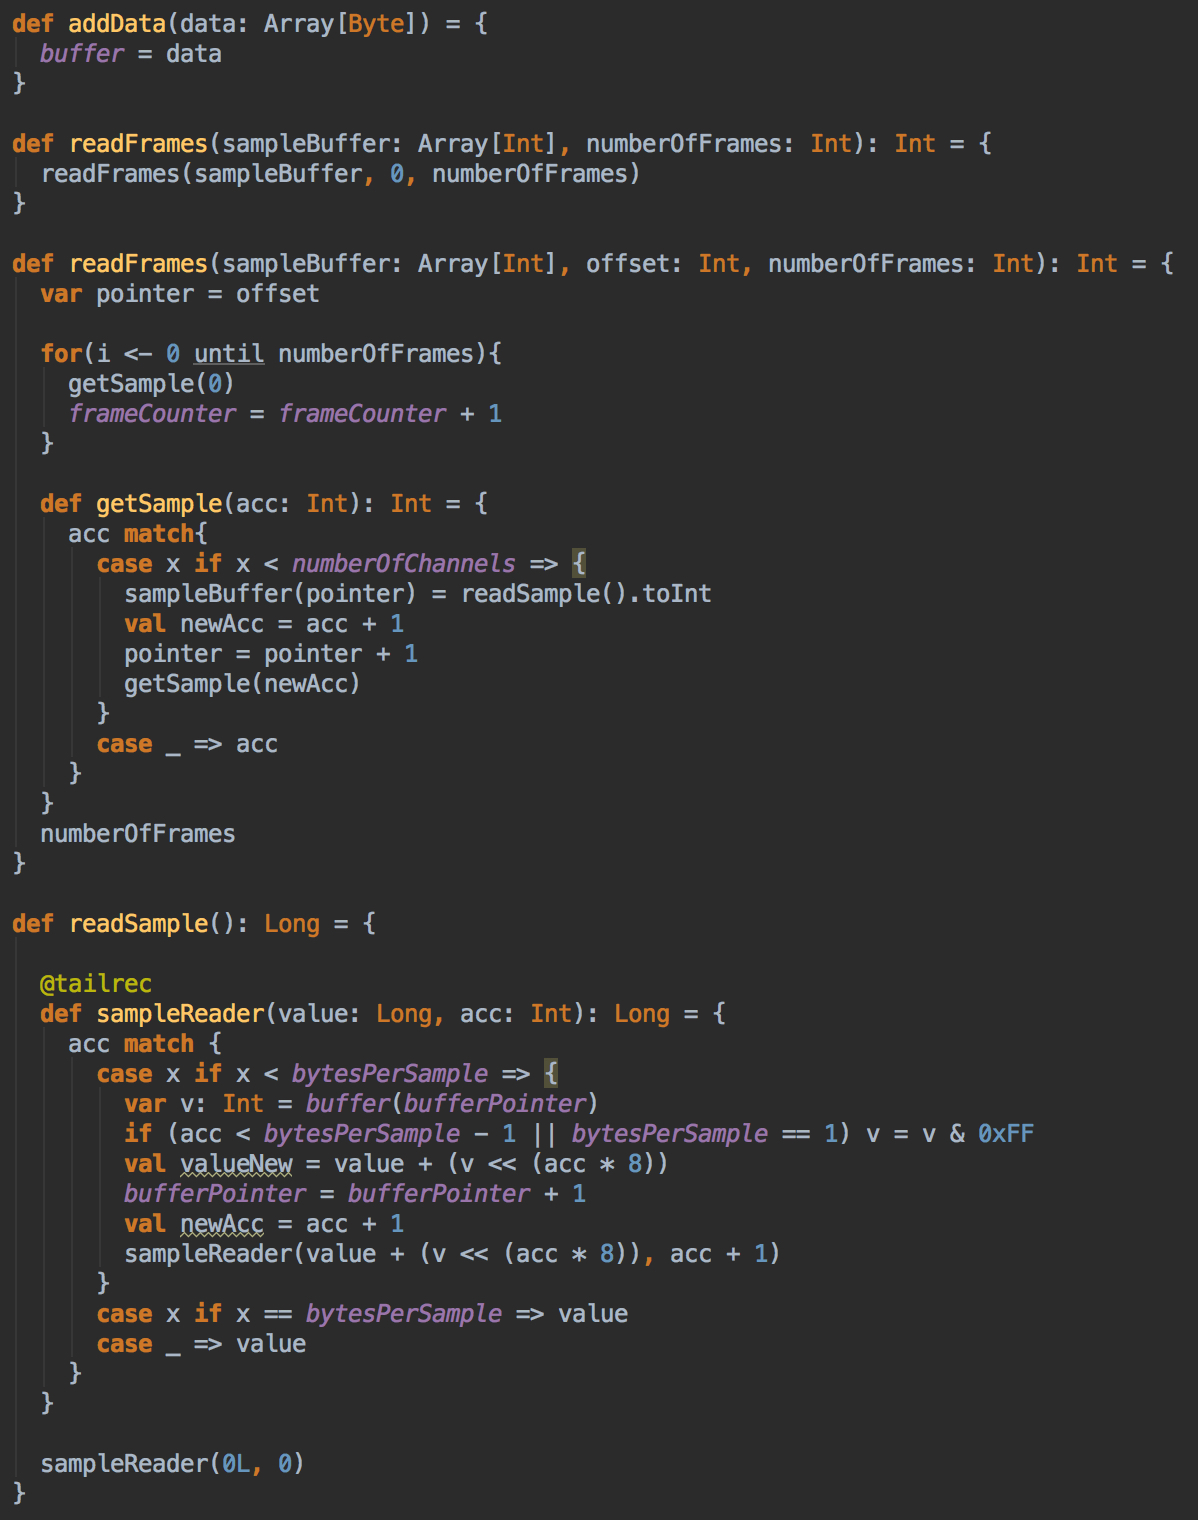
\includegraphics[scale=0.25]{images/liveAudioPro.jpg}
	\caption{LiveAudioProcessor}
	\label{fig: liveAudPro}
\end{figure}

\subsection{Tempo, Analyser, Stats and JSON}
In order for the RTT\_Analyser to be able to process the calculated tempo results the Tempo case class was implemented, comprising of the calculated and expected tempos, and difference between these values, an Option count of beats detected and the time at which the tempo result was calculated. For each tempo result calculates a Tempo object was created and added to a ListBuffer, chosen for its scalability,  within the Analyser implementation corresponding to the relevant beat detection algorithm. The Analyser implementations also contained an Option Stats value, which enabled the Stats to be added to the Analyser after the instantiation of the case class. The Stats case class is used to hold the average and median values of the calculated tempos, as well as the difference between the expected and calcuated tempo. To asses the efficiency of the algorithms the time taken to calculate a tempo within plus or minus one bpm of the expected value. The StatsCalculator case class carried out computation  these which utilised Scala's pattern matching on the List data structure and .. MORE?!

The implementation of the data storage system of the RTT\_Analyser used the JavaScript Object Notation (JSON) as the data generated was considered not large enough to warrant the creation and management of an SQL database. JSON's lightweight data-interchange format\cite{json} ensured the the conversion from Scala case class to JSON object would be straighforward. The JSON was generated the ScalaJSON library provided by the play framework\cite{play}, specifically the \textit{Writes} object which converts an object into a JSON representation held encapsulated within a \textit{JsValue} object. Three methods were written in order to account for the three implementations of the Analyser trait, an example of the code can be seen in Figure(add one). As JSON is written in a text format\cite{json}, the parsing of generated JSON was performed by simpling converting the JSON objects generated by the respective \textit{writes} methods to a string which was then written to a json file using the \textit{flush} method in Figure{add one}, where the path was provided from the user interaction with the RTT\_Analyser's user interface.


\subsection{Adaption of Beatroot}
Once the development of the RTT\_Analyser was considered to be sufficiently on schedule the design decision was taken to attempt the adaption of the Beatroot system to work with live audio again. Much like with the WaveletBPMDetector, Beatroot would have to be set up to use the same audio bytes as those captured by the Performance Worm, to ensure all systems were using the exact same captured audio. As the \textit{AudioWorm} was already set up to capture the enough bytes to work with the WaveletBPMDetector's smallest working window size of 131072, the same figure was chosen to be processed by Beatroot. \par
With the correct design decisions now taken the live audio adaption of Beatroot consisted of only a few minor steps. First, the \textit{processFile} method was amended to receive the byte array holding the audio data recorded by the Performance Worm. A ByteArrayInputStream was then instantiated to hold the data, allowing the \textit{processFrame} and \textit{getFrame} methods to work in the same manner as with a upload static audio file. After the captured audio was processed the ByteArrayInputStream was closed, a step necessary to ensure that no overlap existed between captured audio data sets sent to be processed.

\subsection{The Actor System}
The actor system employed within the RTT\_Analyser is constructed of five different actors in total. The LiveAudioActor assumes the role of the head parent of the system, being responsible for starting and stopping the live audio capture, as well as the termination of the RTT\_Analyser when appropriate. \par

The ProcessingActor, a child of the LiveAudioActor can be considered the coordinator of the storing and processing captured audio data, and the writing of tje calculated tempos. In order to ensure the processing remains as isolated as possible the ProcessingActor employes two worker actors, BeatrootActor and DWTActor, carrying out the two tasks of sending the captured data and tempo calculation. The beat detection worker actors do not return any messages to the ProcessingActor, instead the immutable ActorRef handle which allows for the current instance of the respective actor is passed the respective beat detection system. Therefore, the calculated tempo values are then sent back directly to the ProcessingActor to be stored and subsequently saved to file when appropriate.\par

The final RTT\_Analyser actor was a standalone actor on the same level as the LiveAudioActor within the actor hierachy which was responsible for the timing of the beat detaction test.\par

All of the RTT\_Analyser's parent and child actors were all instantiated in the self contained Operator object. This ensured that potentially dangerous practice of declaring one actor and breaking actor encapsulation\cite{akkaActors} was avoided.  

\subsection{RTT\_Analyser User Interface and HTML Results Viewer}
The RTT\_Analyser's user interface was implemented using the ScalaFX, which sits on the top of the JavaFX API and uses the same declaration syntax as normal objects within Scala. Enabling developers to use the same operators and syntax to create and modify the scene graph\footnote{add one}\cite{scalafx}. It was designed with simplcity in mind. Before starting the user could begin live audio capture the expected bpm, file name and path were required. Once input, there are two modes available to the user. The first is to control the live audio beat detection manually using the start and stop buttons accordingly. The second, is the test mode which will runs the audio capture and beat detection for thirty seconds, before closing down audio inputs and storing the results. During execution the RTT\_Analyser in both of these modes the three calculated tempos are displayed to the user as a bpm value rounded to two decimal places. On completion within both modes the results are stored within a JSON file automatically and also written to an HTML file so the results can be viewed in a web browser using the \textit{Results} button.\par

The HTML tables were produced HtmlWriter object which used reflection where possible to obtain the relevant case class constructor field names, before using a number of tail recursive methods to write the field values and HTML tags to a StringBuilder, chosen for it's mutability. The HTML tables are subsequently saved to an HTML file which is opened and viewed via the default browser using the \textit{Results} button.

\maketitle{}\section{Software Testing}
During the development of the RTT_Analyser, Test Driven Development was employed where possible. TDD is a development process which employs test-first development and refactoring. Test-first development involves writing a test before just enough production code is written to fulfill that test [25]. Refactoring is the process of making small changes to code in order to improve its design, making it easier to understand and modify [26]. I intend to use TDD due to the relatively short development time of this project. TDD will enable small steps to be taken during the process which is considered to be a more productive approach to writing software [25].

\maketitle{}\section{Drum Beat Sample Set and RTT\_Analyser Beat Detection Testing}





\newpage
\begin{thebibliography}{99}
\bibitem{brit-metro} 
\textit{https://www.britannica.com/art/metronome}
\bibitem{drum-bible}
Mick Berry and Jason Gianni\\
\textit{The Drummer's Bible: How to Play Every Drum Style from Afro-Cuban to Zydeco, Second Edition, 2004, See Sharp Press}
\bibitem{oxford-comp}
Alison Latham\\
\textit{The Oxford Companion to Music, 2002, Oxford University Press}
\bibitem{drum-note}
\textit{http://www.drummagazine.com/lessons/post/drumkey/}
\bibitem{allen-danneburg}
Allen and Dannenberg\\
\textit{Tracking Musical Beats in Real Time, International Computer Music Conference, International Computer Music Association, 1990, pp. 140-143}
\bibitem{longeut1}
H. C Longuet-Higgins\\
\textit{Perception of melodies, Nature Vol. 263, 1976, pp. 646-653}
\bibitem{dixon1}
Simon Dixon\\
\textit{Automatic Extraction of Tempo and Beat from Expressive Performances. Journal of New Music Research, 30 (1), 2001, pp 39-58}
\bibitem{dixon2}
Simon Dixon\\
\textit{Onset Detection Revisited, Proceedings of the 9th International Conference on Digital Audio Effects, Montreal, September 2006, pp 133-137}
\bibitem{dixon3}
Simon Dixon\\
\textit{On the Analysis of Musical Expression in Audio Signals. Storage and Retrieval for Media Databases, SPIE-IS\&T Electronic Imaging, SPIE Vol. 5021, 2003 pp 122-132}
\bibitem{mirex-onset}
\textit{http://www.music-ir.org/mirex/wiki/2016:Audio\_Onset\_Detection}
\bibitem{sonic}
\textit{http://www.ieor.berkeley.edu/~ieor170/sp15/files/Intro-to\_Sonic\_Events\_Campion.pdf}
\bibitem{onset-tut}
Juan Pablo Bello, Laurent Daudet, Samer Abdallah, Chris Duxbury, Mike Davies, and Mark B. Sandler 
\textit{A Tutorial on Onset Detection in Music Signals, IEEE TRANSACTIONS ON SPEECH AND AUDIO PROCESSING, VOL. 13, NO. 5, 2005, pp. 1035 - 1047}
\bibitem{mirex-main}
\textit{http://www.music-ir.org/mirex/wiki/2005:Main\_Page}
\bibitem{tzane1}
George Tzanetakis, Georg Essl and Perry Cook\\
\textit{Audio Analysis using the Discrete Wavelet Transform, Proc. WSES International Conference on Acoustics and Music: Theory and Applications (AMTA), 2001}
\bibitem{mirex-06}
\textit{http://www.music-ir.org/mirex/wiki/2006:Audio\_Beat\_Tracking\_Results}
\bibitem{dixon4}
Simon Dixon\\
\textit{Evaluation of the Audio Beat Tracking System BeatRoot. Journal of New Music Research, 36, 1, 2007, pp 39-50}
\bibitem{polikapt2}
\textit{http://users.rowan.edu/ polikar/WAVELETS/WTpart2.html}
\bibitem{lyons}
Lyons\\
\textit{Understanding Digital Signal Processing}
\bibitem{tzane2}
Tao Li, Mitsunori Ogihara, George Tzanetakis\\
\textit{Music Data Mining, CRC Press, 2002, pp 45-53}
\bibitem{tzane3}
George Tzanetakis and Perry Cook\\
\textit{Musical Genre Classification of Audio Signals}
\bibitem{smith}
Steven W. Smith\\
\textit{The Scientist and Engineer's Guide to Digital Signal Processing, California Technical Publishing, 2011, Chapter 3}
\bibitem{pallas}
Ramón Pallás-Areny and John G. Webster\\
\textit{Analog Signal Processing, Wiley, 199, pp. 231}
\bibitem{dixonGoeblWidmer}
Simon Dixon, Werner Goebl and Gerhard Widmer\\
\textit{The Performance Worm: Real Time Visualisation of Expression based on Langner’s Tempo-Loudness Animation, International Computer Music Conference, 16 - 21 September 2002, Göteborg, Sweden, pp 361-364.}
\bibitem{pulseWag}
Bill Waggener\\
\textit{Pulse Code Modulation Techniques}
\bibitem{soundTrail}
Oracle\\
\textit{https://docs.oracle.com/javase/tutorial/sound/}
\bibitem{akkaActors}
Akka\\
\textit{http://doc.akka.io/docs/akka/2.4.9/scala/actors.html}
\bibitem{reactMan}
Jonas Bonér, Dave Farley, Roland Kuhn, and Martin Thompson\\
\textit{Reactive Manifesto, http://www.reactivemanifesto.org/}
\bibitem{acotrsys}
Akka\\
\textit{http://doc.akka.io/docs/akka/2.4.9/general/actor-systems.html}
\bibitem{sbt}
Josh Suereth and Matthew Farwell\\
\textit{SBT in Action: The simple Scala build tool, Manning Publications, 2015}
\bibitem{javasound}
Oracle\\
\textit{https://docs.oracle.com/javase/8/docs/technotes/guides/sound/programmer\_guide/contents.html}
\bibitem{desouze}
\textit{https://github.com/ederwander/Beat-Track}
\bibitem{marcoZin}
\textit{https://github.com/mziccard/scala-audio-file}
\bibitem{green}
Andrew Greensted
\textit{http://www.labbookpages.co.uk/audio/javaWavFiles.html}
\bibitem{mariusEr}
Marius Eriksen\\
\textit{Effective Scala, http://twitter.github.io/effectivescala/}
\bibitem{odesky}
Martin Odersky, Lex Spoon and Bill Venners\\
\textit{Programming in Scala, Second Edition, Artima Press, 2010}
\bibitem{play}
\textit{https://www.playframework.com/documentation/2.5.x/ScalaJson}
\bibitem{json}
\textit{http://www.json.org/}
\bibitem{play-writes}
\textit{https://www.playframework.com/documentation/2.5.x/api/scala/index.html\#play.api.libs.json.Writes}
\bibitem{scalafx}
\textit{http://www.scalafx.org/docs/home/}
\end{thebibliography}
\end{document}



